\documentclass[12pt]{scrartcl}
\usepackage[hidelinks]{hyperref}
\usepackage[utf8]{inputenc}
\usepackage{graphicx}
\usepackage{mathtools}
\usepackage[]{algorithmic}
\usepackage[]{algorithm}


\begin{document}
\renewcommand{\algorithmicrequire}{\textbf{Input:}}
\renewcommand{\algorithmicensure}{\textbf{Output:}}
\renewcommand{\algorithmicforall}{\textbf{for each}}

\section*{Proof Sketch}
It is assumed that the stages of pairs finding, disks generation and `\textit{less-than-$\mu$}' disk filtering have already been done. We start with a set of candidate disks which are represented by their centers and the set of original points which are enclosed by them.  It is expected that they are organized in an R-Tree index as it is shown in figure \ref{fig:r-tree}.  The following procedure aims to filter out candidate disks when its set of points is a subset of another disk's set of points.  Just disks with a superset of points are kept and they are known as maximal disks. 

\begin{figure}
  \centering
  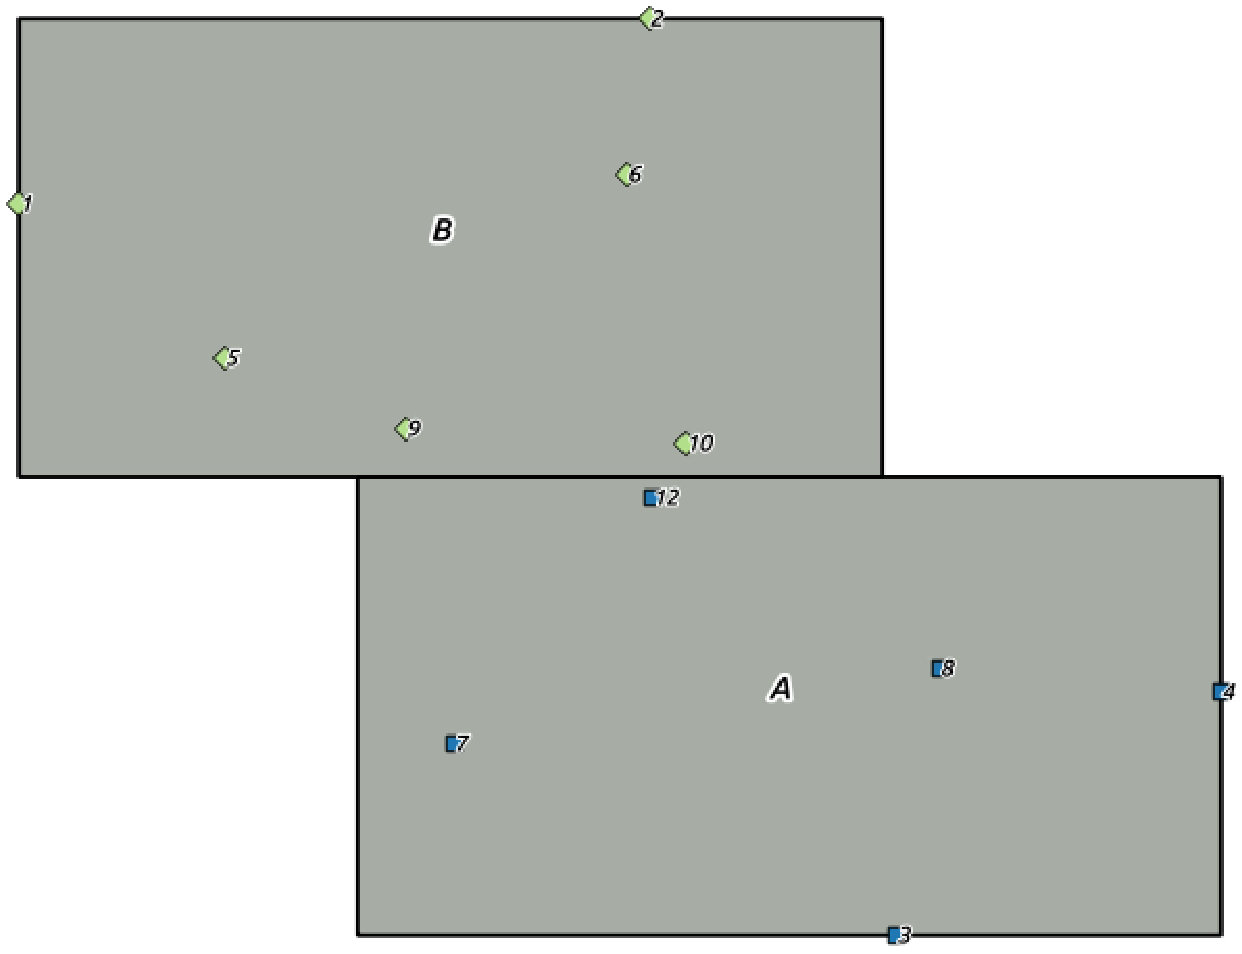
\includegraphics[width=0.7\textwidth]{./Figures/r-tree}
  % R-Tree.png: 0x0 pixel, 300dpi, 0.00x0.00 cm, bb=
  \caption{An inital R-Tree over a set of candidates disks represented by their centers.}
  \label{fig:r-tree}
\end{figure}

There are two problems during the filtering and report of maximal disks following a parallel approach. First, it can be disks with the same set of points which are reported as maximals in different partitions.  We should report only one of them.  Second, it can be a disk with a subset of points which appears as a maximal disk in one partition but there is another disk in another partition with a superset of points that contains that set.   We should just report the disk containing the superset.  We will refer the first problem as \textit{duplicate reporting} and the second one as \textit{subset reporting}.  

Duplicate reporting can be easily avoided by using a deterministic way to represent the center of each disk previous to the partitioning.  It is, using an unique center for those disks with the same set of points.  For example, changing the center of the disks to the MBR's centroid their points will lead to a unique representation of the disks.  Note that the change of the center's location does not affect the logic of the procedure due to the set of points of the disks remains the same.

Subset reporting demands more attention.  In order to avoid this problem, we have to evaluate disks which potentially can contain the set of points of other disks.  Keep in mind that just disks which intersect each other should be evaluated as that means that they have points in common. From figure \ref{fig:r-tree}, it is clear than disks close to the edge of each partition\footnote{In this context, we refer to partition or MBR indistinctly.} could intersect other disks in the edge of contiguous partitions. Specifically, disks lying $\epsilon$ distance to the edge of their MBRs must be further analyzed but note that those remaining in the internal area are certainly safe. 

\begin{figure}
	\centering
	\begin{center}
	\includegraphics[width=0.8\textwidth]{./Figures/expansion}
	% R-Tree.png: 0x0 pixel, 300dpi, 0.00x0.00 cm, bb=
\end{center}
	\caption{An $\epsilon$ expansion over the partitions of the R-Tree. Note that just disks in the expansion areas which intersect each other should be further analyzed. }
	\label{fig:expansion}
\end{figure}

As we have access to the R-Tree's MBRs, we perform an expansion applying a $\epsilon$ buffer around each of them (see figure \ref{fig:expansion}). As the radius of each disk is $\frac{\epsilon}{2}$, it is clear that a disk in any specific partition only can intersect other disks if they lie in the expansion area of its partition.  

We re-index the original set of candidate disks using the new expanded MBRs.  For those disks which intersect multiple expanded MBRs, a copy of the disk is sent to each of them. If a disk lie in the expansion area of one of the new MBR, it is marked accordingly. A disk can lie in the expansion area of multiple MBRs but it will be outside of the expansion area of its original MBR. 

Now we can run a maximal pattern algorithm to find supersets of points and their correspond disks in each partition. Any candidate disk with a subset of points will be obfuscated by its superset (if any) lying in the expansion area avoiding subset reporting.  In order to avoid duplicate reporting, caused by copy of disks during expansion, we only report a maximal disk if it does not lie in the expansion area. As a disk will only be one time outside of an expansion area, we let this disk to be reported by its original partition.

\clearpage

\begin{algorithm}
  \footnotesize
  \caption{Finding maximal disks following a parallel approach.}
  \label{alg:maximals}
  \begin{algorithmic}
    \REQUIRE 
    Set of points $T$, maximum distance $\epsilon$ and minimum size $\mu$ \\

    \ENSURE 
    Set of maximal disks $M$ 
    \vspace{3mm}
    % 01.Indexing points... 
    % 02.Getting pairs... 
    \STATE find the set of pairs of points $P$ in $T$ which are $\epsilon$ distance each other
    % 03.Computing centers... 
    \STATE $C \leftarrow$ \O{}
    \FORALL{$p_i$ in $P$}
      \STATE compute disks $c_i^1$ and $c_i^2$ of $p_i$ using $\epsilon$ 
      \STATE add $c_i^1$ and $c_i^2$ to $C$
    \ENDFOR
    % 04.Indexing centers... 
    % 05.Getting disks... 
    \STATE $D \leftarrow$ \O{}
    \FORALL{$c_i$ in $C$} 
      \STATE find the set of points $\rho_i$ which lie $\epsilon$ distance around $c_i$ 
      \IF{$|\rho_i| \geq \mu$} % 06.Filtering less-than-mu disks... 
		\STATE compute centroid $\varsigma_i$ of the MBR of $\rho_i$ 
		\STATE set $d_i.center$ as $\varsigma_i$
		\STATE set $d_i.points$ as $\rho_i$
		\IF{$d_i$ not in $D$}
			% 07.Prunning duplicate candidates...
			\STATE add $d_i$ to $D$ \COMMENT{Prunning duplicate candidates...} 
		\ENDIF
      \ENDIF
    \ENDFOR
    % 08.Indexing candidates...
    \STATE build an R-Tree $disksRT$ using centers in $D$ 
    % 09.Getting expansions... 
    \STATE $E \leftarrow$ \O{}
	\FORALL{MBR in $disksRT$} 
		\STATE expand MBR to create an expanded MBR $\varepsilon_i$ using a buffer of $\epsilon$ distance 
		\STATE add $\varepsilon_i$ to $E$
	\ENDFOR
	\FORALL{$d_i$ in $D$}
		\FORALL{$\varepsilon_j$ in $E$}
			\IF{$d_i.center \cap \varepsilon_j$}
				\STATE add $d_i$ to $\varepsilon_j$ 
			\ENDIF
		\ENDFOR
	\ENDFOR
    % 10.Finding maximal disks...
    \STATE $M \leftarrow$ \O{}
    \FORALL{$\varepsilon_i$ in $E$} 
		\STATE $\chi \leftarrow$ \O{} 
		\FORALL{$d_i$ in $\varepsilon_i$}
			\STATE add $d_i.points$ to $\chi$
		\ENDFOR
		\STATE find the set of maximal patterns $F$ in $\chi$
		\FORALL{$f_i$ in $F$}
			\STATE compute centroid $\varsigma_i$ of the items in $f_i$
			\IF{$\varsigma_i$ is not in the expansion area of $\varepsilon_i$}
				\STATE set $m_i.center$ as $\varsigma_i$
				\STATE set $m_i.points$ as $f_i$
				\STATE add $m_i$ to $M$
			\ENDIF
		\ENDFOR
	\ENDFOR
	
	\RETURN M
  \end{algorithmic}
\end{algorithm}

\end{document}
